\chapter{Experiment Result and Analysis}
\label{Chapter4}
\section{Experimental Setting}
\subsection{Evaluation metric}
In this study, we employ a range of evaluation metrics to assess the effectiveness of our algorithms.

\begin{itemize}
	\item $l_1$ norm accuracy 
	\begin{equation}
		l_1(f,g) = \int |f(x)-g(x)|dx.
	\end{equation}
	\begin{equation}
		\text{Acc}(f,g) = 1 - \frac{1}{2}l_1(f,g). 
	\end{equation}
	\item Run time: This metric represents the total time (in seconds) taken to generate the posterior density.
	
\end{itemize}
The $l_1$ norm is commonly employed to compare probability densities, particularly to assess the accuracy of the distribution's central tendency. The emphasis on calculating $l_1$ norm accuracy stems from the recognition that the accuracy of the tail distribution approximation is relatively less significant compared to that of the central distribution. The primary objective of our approximation for the posterior distribution centers around achieving precision in the central region.
Additionally, it is important to evaluate the execution time required for generating posterior parameters. This examination allows for a comprehensive comparison of time complexity among the Local-Global algorithm, MFVB, and MCMC methods. The execution time is measured in seconds.
%Objective: Use math to find a posterior mode of lasso distribution: Given a,b,c
%Task: Check if the posterior estimate reach 
%Metric: Use Posterior TP/FP Rate(Soft thresholding operator) Check if a local parameter mode is close to 0, compared with true parameters, and use this for 
%Variable Selection
%
%Expectation: posterior mode sparse, posterior mean not sparse

\subsection{Experimental Datasets}
The following bullet points demonstrate the dataset description, which includes the introduction to the purpose of the dataset, and a number of predictors and number of samples, respectively.
\begin{itemize}
	
	\item \textbf{Hitters}:
	\begin{itemize}
		\item Type: Baseball statistics dataset
		\item Predictors ($p$): 20, Samples ($n$): 263
		\item Description: Contains baseball player statistics, including performance measures and salary information.
		\item Further description: High correlation between predictors
	\end{itemize}
	
	\item \textbf{Kakadu}:
	\begin{itemize}
		\item Type: Environmental dataset
		% ????????
		\item Predictors ($p$): 22, Samples ($n$): 1828
		\item Description: Relates environmental factors to the abundance of amphibians in Kakadu National Park, Australia.
		\item Further description: Approximately normal posterior distribution due to large number of samples.
	\end{itemize}
	
	\item \textbf{Bodyfat}:
	\begin{itemize}
		\item Type: Human body measurements dataset
		\item Predictors ($p$): 15, Samples ($n$): 250
		\item Description: Contains measurements of various body parts for a sample of individuals, such as weight, height, and circumferences.
		\item Further description: Approximately normal distribution,   strong correlation between predictors.
	\end{itemize}
	\item \textbf{Prostate}:
	\begin{itemize}
		\item Type: Medical dataset
		\item Predictors ($p$): 8, Samples ($n$): 97
		\item Description: Prostate cancer data with clinical measurements and Logarithm of Prostate Specific Antigen (lpsa).
		\item Further description: Approximately normal posterior distribution, no strong correlation between predictors.
	\end{itemize}
	
	\item \textbf{Credit}:
	\begin{itemize}
		\item Type: Credit scoring dataset
		\item Predictors($p$): 11, Samples ($n$): 400
		\item Description: Contains information about loan applicants, such as credit history, employment, and demographics, to assess creditworthiness.
		\item Further description: Approximately normal posterior distribution, no strong correlation between predictors.
	\end{itemize}
	
	\item \textbf{Eye data}:
	\begin{itemize}
		\item Type: Medical dataset
		\item Predictors ($p$): 200, Samples ($n$): 120
		\item Description: Contains measurements related to glaucoma patients, such as intraocular pressure and visual acuity, to assess the effectiveness of treatment options.
		\item Further description: The number of predictors is higher than the sample size.
	\end{itemize}
\end{itemize}
In particular, the Hitters dataset and Eye data dataset deserve additional attention due to their distinct characteristics. Hitters exhibits a substantial correlation among predictors, while Eyedata possesses a larger number of predictors compared to the number of samples, making both datasets more challenging to approximate accurately. However, if the Local-Global algorithm can achieve higher accuracy and better approximation density than MFVB on these challenging datasets, it suggests that the algorithm's success can extend to other datasets that are comparatively easier to approximate. The experimental results, which will be presented in a later subsection, will primarily focus on Hitters and Eye data while also comparing the findings to those obtained from other datasets.

\section{Experimental Result}
\subsection{Approximation Density Visualization}
The following six plots illustrate the approximated density plots for each of the datasets. Since each dataset contains a large number of predictors, we will present two density plots for each dataset. The first plot represents the best density approximation achieved by the Local-Global algorithm with MCMC, while the second plot represents the worst density approximation, exhibiting the largest deviation from MCMC. To enhance readability, the best plot will be positioned on the left, and the worst plot will be placed on the right.\\
Regarding the density plots for the Kakadu, Prostate, Bodyfat, and Credit datasets, there are no significant deviations observed between the density plots generated by MFVB, Local-Global Global (LG-Global) approximation, and Local-Global Local (LG-Local) approximation with MCMC. The predictors in these datasets generally demonstrate a roughly normal density pattern. As a result, the approximation accuracy for MFVB remains relatively high, whereas LG-Local and LG-Global may experience a more noticeable decrease in approximation accuracy due to the distinctive characteristics of these datasets.\\
\newpage
% Define what is worst and best??
\begin{figure}[h]
	\begin{subfigure}{0.5\textwidth}
		\centering
		\includegraphics[page = 15, width=\linewidth,keepaspectratio]{lasso_densities_Hitters.pdf}
	\end{subfigure}
	\begin{subfigure}{0.5\textwidth}
		\includegraphics[page = 8, width=\linewidth,keepaspectratio]{lasso_densities_Hitters-1.pdf}
	\end{subfigure}
	\caption{Part of Approximation Density for Hitters dataset; Left: best case, Right: worst case}
	\label{fig:hitters1}
\end{figure}

In \autoref{fig:hitters1}, the density plot of this particular predictor reveals significant overlap with the MCMC plot, as shown on the left-hand side. This overlap indicates a high level of accuracy in the approximation performance.

In contrast, when examining the worst density plot, it is observed that MFVB tends to deviate from the left-skewed MCMC (considered as the gold standard). Particularly in scenarios where the actual distribution possesses a sharp tuning point, both the local and global algorithms, particularly the local approximation line, demonstrate a closer approximation to the gold standard. This improved performance can be attributed to the inclusion of the absolute term $c|x|$ in the lasso distribution formula, which allows for accommodating various potential density functions.
\newpage
\begin{figure}[h]
	\begin{subfigure}{0.5\textwidth}
		\centering
		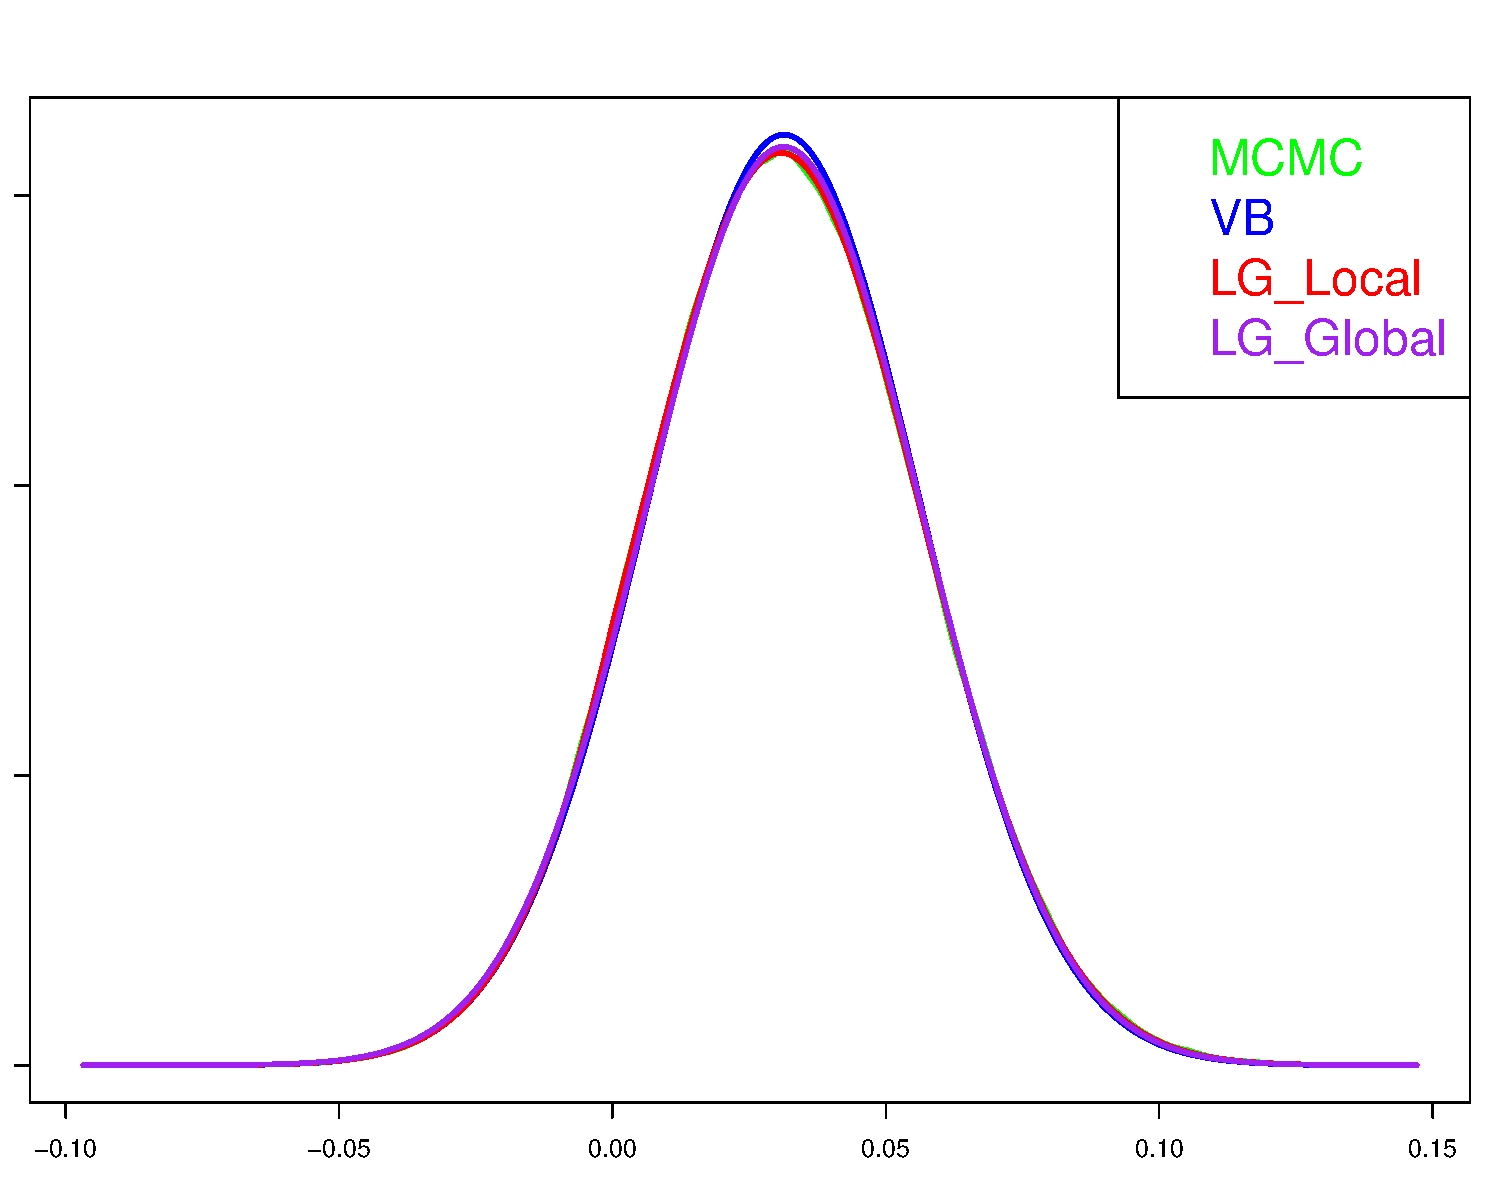
\includegraphics[page = 1, width=\linewidth,keepaspectratio]{lasso_densities_Kakadu.pdf}
	\end{subfigure}
	\begin{subfigure}{0.5\textwidth}
		\includegraphics[page = 2, width=\linewidth,keepaspectratio]{lasso_densities_Kakadu-1.pdf}
	\end{subfigure}
	\caption{Part of Approximation Density for Kakadu dataset; Left: best case, Right: worst case}
	\label{fig:Kakadu}
\end{figure}

In \autoref{fig:Kakadu}, the best density plot obtained from the Local-Global algorithms exhibits significant overlap with both MCMC and MFVB, similar to the findings in \autoref{fig:hitters1}. In the worst-case scenario, LG-Local continues to demonstrate the best approximation performance. Despite the gold standard density displaying high variance, LG-Local manages to fit a density with a comparable variance, even in the presence of a sharp tuning point.\\
\begin{figure}[h]
	\begin{subfigure}{0.5\textwidth}
		\centering
		\includegraphics[page = 1, width=\linewidth,keepaspectratio]{lasso_densities_Bodyfat.pdf}
	\end{subfigure}
	\begin{subfigure}{0.5\textwidth}
		\includegraphics[page = 8, width=\linewidth,keepaspectratio]{lasso_densities_Bodyfat-1.pdf}
	\end{subfigure}
	\caption{Part of Approximation Density for Bodyfat dataset; Left: best case, Right: worst case}
	\label{fig:Bodyfat}
\end{figure}

In \autoref{fig:Bodyfat}, the best density plot obtained from the Local-Global algorithms exhibits significant overlap with both MCMC and MFVB. This overlap is attributed to the dataset itself, which demonstrates an asymptotically normal data distribution, similar to the case mentioned earlier. Furthermore, under the worst-case scenario, LG-Local continues to showcase the best approximation performance, as shown on the right side of \autoref{fig:Bodyfat}. The LG-Local line aligns closely with the density plot generated by the gold standard, represented by the green line.

\begin{figure}[h]
	\begin{subfigure}{0.5\textwidth}
		\centering
		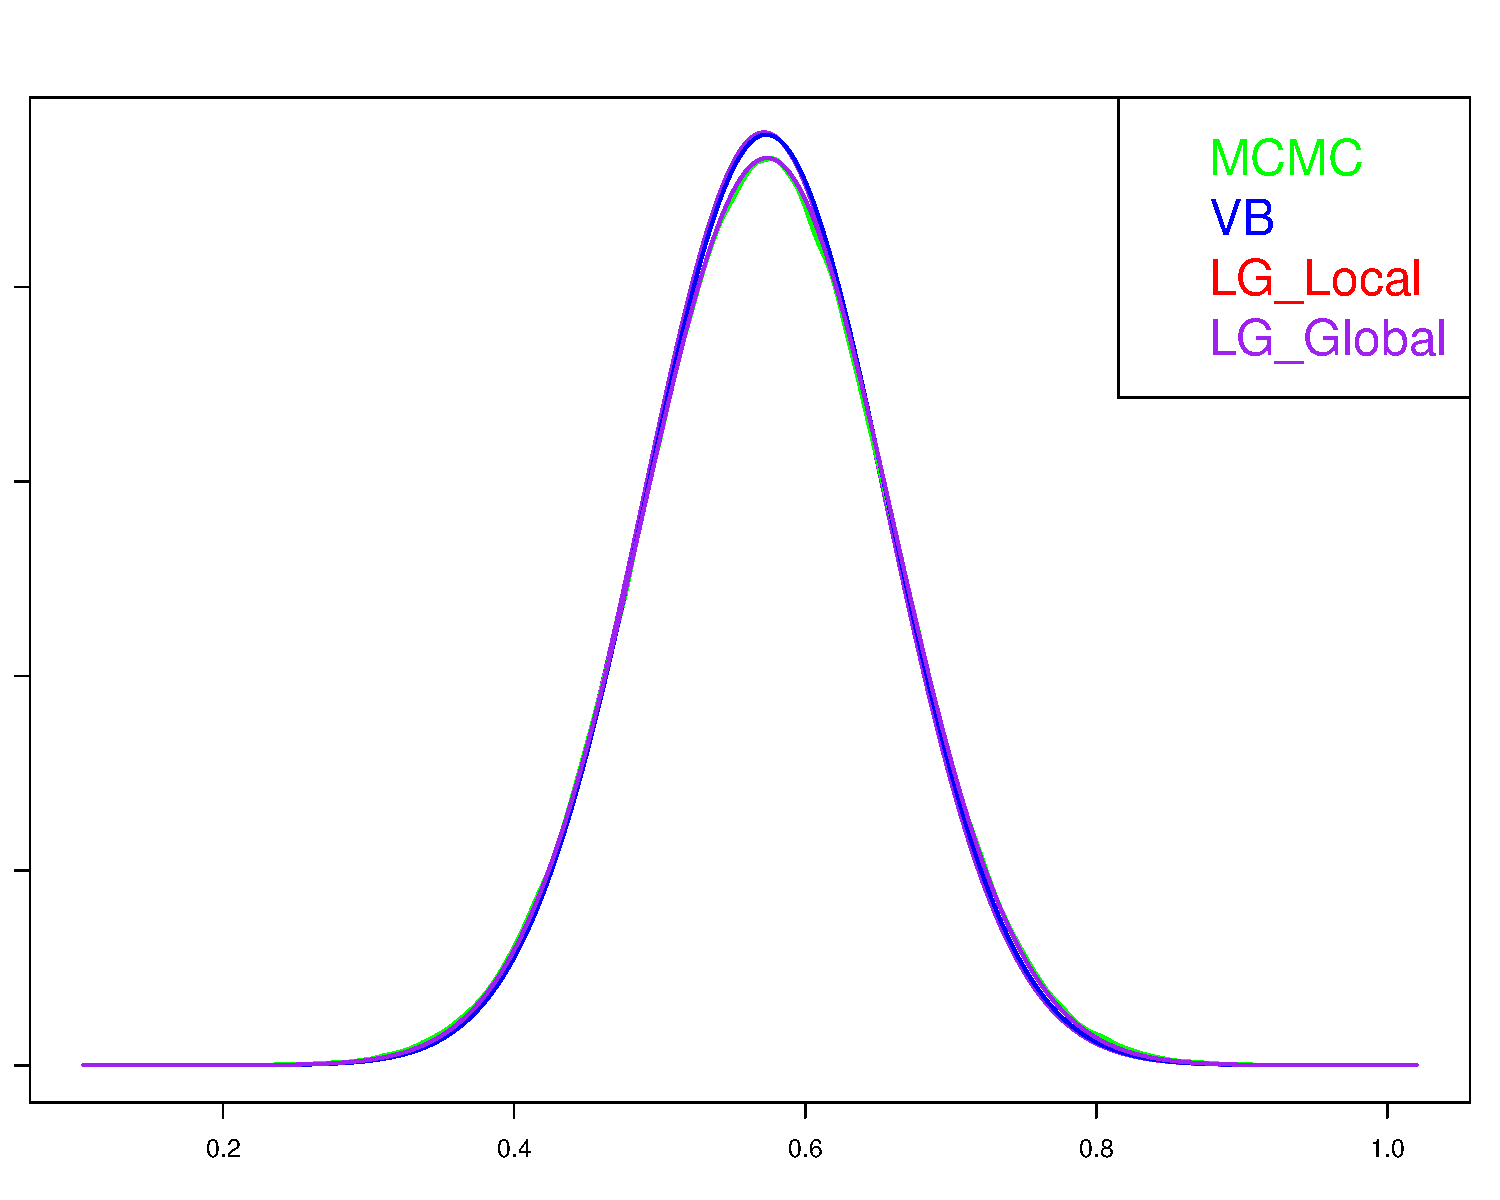
\includegraphics[page = 1, width=\linewidth,keepaspectratio]{lasso_densities_prostate.pdf}
	\end{subfigure}
	\begin{subfigure}{0.5\textwidth}
		\includegraphics[page = 7, width=\linewidth,keepaspectratio]{lasso_densities_prostate-1.pdf}
	\end{subfigure}
	\caption{Part of Approximation Density for Prostate dataset; Left: best case, Right: worst case}
	\label{fig:Prostate}
\end{figure}
In the best-case scenario depicted in \autoref{fig:Prostate}, MFVB slightly overestimates the posterior variance. However, both LG-local and LG-global exhibit high robustness against the target distribution, accurately capturing its characteristics.

On the other hand, in the worst-case scenario, while LG-global moderately underestimates the posterior variance, LG-local demonstrates once again its consistency with MCMC, accurately reflecting the distribution's properties.

\begin{figure}[h]
	\begin{subfigure}{0.5\textwidth}
		\centering
		\includegraphics[page = 11, width=\linewidth,keepaspectratio]{lasso_densities_Credit.pdf}
	\end{subfigure}
	\begin{subfigure}{0.5\textwidth}
		\includegraphics[page = 2, width=\linewidth,keepaspectratio]{lasso_densities_Credit-1.pdf}
	\end{subfigure}
	\caption{Part of Approximation Density for Credit dataset; Left: best case, Right: worst case}
	\label{fig:Credit}
\end{figure}

In a similar fashion to previous observations, the Local-Global approximation exhibits significant overlap with both MFVB and MCMC, as illustrated on the left side of \autoref{fig:Credit}.

In the worst-case plot, MFVB tends to overestimate the posterior variance. However, both LG-local and LG-global demonstrate a remarkable alignment with the MCMC density plot, indicating their ability to accurately capture the distribution's characteristics.

\begin{figure}[h]
	\begin{subfigure}{0.5\textwidth}
		\centering
		\includegraphics[page = 52, width=\linewidth,keepaspectratio]{lasso_densities_eyedata-1.pdf}
	\end{subfigure}
	\begin{subfigure}{0.5\textwidth}
		\includegraphics[page = 200, width=\linewidth,keepaspectratio]{lasso_densities_eyedata.pdf}
	\end{subfigure}
	\caption{Part of Approximation Density for Eyedata dataset; Left: best case from 52nd predictor, Right: worst case from 200th predictor}
	\label{fig:Eyedata}
\end{figure}

In the best scenario depicted on the left side of \autoref{fig:Eyedata}, the most significant distinction is observed. This is due to the fact that, for a majority of predictors in the Eyedata dataset, the actual distribution, as represented by the MCMC plot, does not follow an asymptotically normal pattern. As a result, the optimal approximation case displays a Laplacian-like distribution. This deviation from the assumed distribution can directly lead to inaccurate results for both MFVB and LG-Global.

In the worst-case scenario shown on the right side of \autoref{fig:Eyedata}, the marginal LG-local approximation slightly underestimates the data distribution, but overall, it still outperforms the other two plots. MFVB approximation, on the other hand, considerably overestimates the posterior variance once again.

Although the assumption of normal distribution exists for LG-Global, it tends to correct the overestimated posterior variance of the regression coefficient when compared with MFVB. 

\subsection{Approximation Accuracy Result}
The following six tables present the experimental results for the approximation accuracy of three different algorithms. LG-Local represents the marginal approximation of the Local-Global Algorithm using the lasso distribution, while LG-Global represents the global approximation of the Local-Global Algorithm using a univariate normal distribution. The global mean for LG-Global is set at the $j_{th}$ component, and the variance is determined by the $j_{th}$ row and $j_{th}$ column of $\tilde{\Sigma}$.

Each row in the tables corresponds to a specific quantile of approximation accuracy, such as the minimum approximation accuracy, maximum approximation accuracy, and so on. LG-Local reflects the local approximation accuracy achieved by our algorithm, while LG-Global represents the global approximation accuracy. The VB column denotes the Mean-Field-Variational-Bayes algorithm, and the MCMC column refers to the Monte Carlo Markov Chain method, which serves as a gold standard with 100\% accuracy for each approximation density.


\begin{table}[!h]
	\resizebox{\linewidth}{!}{
		\begin{tabular}{|p{3cm}||c| c| c|c|c|c|}
			\hline
			Algorithm  & MCMC  & VB & LG\_Local & LG\_Global \\
			\hline
			Min.   &   100 & 86.8     &  97.3   &   89.3\\
			1st Qu. &  100 & 92.1  &   99.2  &    97.0\\
			Median &  100 & 95.7     &  99.6   &   97.4\\
			Mean  &   100 & 94.2   &  99.3  &    97.1\\
			3rd Qu.&  100 &  97.4     &  99.7  &    99.0\\
			Max.  &   100 & 98.7    &  99.8   &   99.7\\
			Run Time(s) &  453.75  & 0.17  & 0.17  & 0.17 \\
			\hline
	\end{tabular}}
	\caption{Experiment Result on Hitters dataset}
	\label{table:Hitter}
\end{table}

Table \ref{table:Hitter} presents the approximation results for the Hitters dataset. The global approximation of the Local-Global algorithm outperforms the benchmark approach, MFVB, across all metrics by approximately 1 to 5 percent. The running time of the Local-Global algorithm is 0.17s, which is 0.03s slower than MFVB. This is expected as MFVB only involves the global parameter approximation, without the additional step of local approximation. Furthermore, both methods are 400 times faster than MCMC.

The Local-Global algorithm demonstrates superior approximation accuracy in this particular dataset, which is considered the most challenging among all the datasets, without a significant increase in running speed.


\begin{table}[!h]
	\resizebox{\linewidth}{!}{
		\begin{tabular}{|p{3cm}||c| c| c|c|c|c|}
			\hline
			Algorithm  & MCMC  & VB & LG\_Local & LG\_Global \\
			\hline
			Min.   &  100 &93.2    &   95.9    &  92.2\\
			1st Qu.&  100 & 98.9  &    99.8   &   99.2\\
			Median &  100 & 99.2    &   99.8   &   99.4\\
			Mean   &  100 &  98.6  &    99.4 &     98.8\\
			3rd Qu.&  100 & 99.3  &   99.8 &     99.8\\
			Max.   &  100 & 99.7  &   99.8  &    99.8\\
			Run Time(s) &6696.56 & 0.14 &0.19 & 0.19\\
			\hline
	\end{tabular}}
	\caption{Experiment Result on Kakadu dataset}
	\label{table:Kakadu}
\end{table}

Table \ref{table:Kakadu} presents the approximation results for the Kakadu dataset. While the minimum global approximation of the Local-Global algorithm is lower than MFVB, all other metrics show slightly higher values for the Local-Global algorithm. Regarding the local approximation, LG-Local, there is a one to two percentage increase compared to MFVB. Additionally, the execution time for the Local-Global algorithm is 0.05s shorter than that of MFVB (0.14s). Both methods achieve a speed that is 6000 times faster than that of MCMC. This significant speed improvement is due to the high number of samples in the Kakadu dataset, which requires a longer running time for MCMC sampling.
Despite the longer execution time required for MCMC, the performance of both the MFVB method and the Local-Global algorithm does not degrade significantly because the data distribution in Kakadu is approximately normal.

\begin{table}[!h]
	\resizebox{\linewidth}{!}{
		\begin{tabular}{|p{3cm}||c| c|c| c|c|c|c|}
			\hline
			Algorithm  & MCMC  & VB & LG\_Local & LG\_Global \\
			\hline
			Min.   &  100  & 91.3     &   96.3  &     90.7\\
			1st Qu. & 100  & 97.0      &  99.6   &    97.6\\
			Median  &  100  & 98.0    &   99.7  &     98.4\\
			Mean    &  100 &  97.0     &   99.2   &    97.2\\
			3rd Qu.  & 100  &  98.4      &   99.7  &     98.6\\
			Max.    &  100 & 99.3    &   99.7    &   99.7\\
			Run Time(s) &  398.59  & 0.14   & 0.17  & 0.17 \\
			\hline
	\end{tabular}}
	\caption{Experiment Result on bodyfat dataset}
	\label{table:bodyfat}
\end{table}

Table \ref{table:bodyfat} presents the approximation results for the Bodyfat dataset. Similar to the Kakadu dataset, the minimum global approximation of the Local-Global algorithm is lower than MFVB, while all other metrics show slightly higher values for the Local-Global algorithm. In terms of the local approximation, LG-Local, there is a 2 to 5 percent increase compared to MFVB. Moreover, the execution time for the Local-Global algorithm is 0.03s shorter than that of MFVB (0.14s). Both methods achieve a speed that is 300 times faster than that of MCMC.

The data distribution in the Bodyfat dataset is similar to that of the Kakadu dataset, resulting in no drastic difference between MFVB and the Local-Global algorithm.

\begin{table}[!h]
	\resizebox{\linewidth}{!}{
		\begin{tabular}{|p{3cm}||c| c|c| c|c|c|c|}
			\hline
			Algorithm  & MCMC  & VB & LG\_Local & LG\_Global \\
			\hline
			Min.  &   100& 96.9 &    99.5   &   97.4\\
			1st Qu. & 100& 97.2 &    99.5   &   97.9\\
			Median &  100& 97.6  &    99.6   &   98.9\\
			Mean  &   100& 97.5  &    99.6  &    98.7\\
			3rd Qu.&  100& 97.7   &   99.6  &    99.5\\
			Max.   &  100& 98.4  &    99.6  &    99.6\\
			Run Time(s) &  336.31  & 0.11  & 0.12  & 0.12 \\
			\hline
	\end{tabular}}
	\caption{Experiment Result on Prostate dataset}
	\label{table:prostate}
\end{table}

Table \ref{table:prostate} presents the approximation results for the Prostate dataset. Similar to the Kakadu and Bodyfat datasets, the global approximation of the Local-Global algorithm is slightly higher than MFVB. Additionally, the local approximation accuracy of LG-Local surpasses both the global approximation and MFVB.

In terms of execution time, the Local-Global algorithm is 0.01s faster than MFVB (0.11s), and both methods achieve a speed that is 300 times faster than that of MCMC.

The data distribution in the Prostate dataset is similar to that of the Bodyfat and Kakadu datasets, with an approximately normal distribution. Consequently, there is no significant distinction between the performance of MFVB and the Local-Global algorithm in this dataset.

\begin{table}[!h]
	\resizebox{\linewidth}{!}{
		\small
		\begin{tabular}{|p{3cm}||c| c|c| c|c|c|c|}
			\hline
			Algorithm  & MCMC  & VB & LG\_Local & LG\_Global \\
			\hline
			Min.   &  100& 91.8   &   99.5   &   99.3\\
			1st Qu. & 100& 98.3 &    99.7   &   99.5\\
			Median &  100& 99.4   &   99.8   &   99.5\\
			Mean   &  100& 97.9   &   99.7   &   99.6\\
			3rd Qu.&  100 & 99.5   &  99.8   &   99.7\\
			Max.  &   100 & 99.7   &    99.8   &   99.8\\
			Run Time(s) &  359.92  & 0.1  & 0.11  & 0.11 \\
			\hline
	\end{tabular}}
	\caption{Experiment Result on Credit dataset}
	\label{table:Credit}
\end{table}

Table \ref{table:Credit} showcases the approximation results for the Credit dataset. Similar to the Prostate dataset, the global approximation of the Local-Global algorithm is slightly higher than MFVB, although the minimum value of MFVB is approximately 8\% lower than LG-Global. Both LG-Global and LG-Local achieve an approximation accuracy above 99\%.

In terms of execution time, the Local-Global algorithm requires 0.11s, which is only 0.01s slower than the Local-Global Algorithm. Both methods achieve a speed that is 300 times faster than that of MCMC.

It is worth noting that the Credit dataset, like the Prostate, Bodyfat, and Kakadu datasets, exhibits properties of a roughly normal distribution. Consequently, the results obtained align with the findings from the previous datasets.


\begin{table}[!h]
	\resizebox{\linewidth}{!}{
		\small
		\begin{tabular}{|p{3cm}||c| c|c| c|c|c|c|}
			\hline
			Algorithm  & MCMC  & VB & LG\_Local & LG\_Global \\
			\hline
			Min.    & 100 & 78.4   &   97.3   &   86.1\\
			1st Qu. & 100 & 86.9   &   98.6   &   90.4\\
			Median &  100 & 90.3   &   98.7  &    91.3\\
			Mean   & 100 & 88.9  &   98.7  &    91.8\\
			3rd Qu. & 100 &91.2    &  98.8   &   92.3\\
			Max.   &  100 &93.1  &   99.1  &    99.2\\
			Run Time(s) &  18144.7  & 1.21  & 1.72  & 1.72 \\
			\hline
	\end{tabular}}
	\caption{Experiment Result on Eyedata dataset}
	\label{table:Eyedata}
\end{table}


Table \ref{table:Eyedata} presents the approximation results for the Eyedata dataset. The global approximation of the Local-Global algorithm surpasses that of MFVB by a significant margin. Furthermore, the local approximation accuracy of LG-Local is notably higher than both the global approximation and MFVB.

In terms of execution time, the Local-Global algorithm is 0.51s faster than MFVB (1.21s). Both methods achieve a speed that is 18000 times faster than that of MCMC.

It is important to highlight the unique characteristic of the Eyedata dataset, namely its high-dimensional sparsity. The curse of dimensionality poses challenges to the approximation process, particularly for MCMC, which requires more steps to converge. In this case, although MFVB offers slightly faster execution, the Local-Global algorithm demonstrates a more robust performance in terms of approximation accuracy.






